\chapter{Introduction}
\label{cha:introduction}

\section{Background}
\label{sec:Background}

Translation of findings from genomics study to inform medical practices is a highly important research area. Genomics suggests disease onset and therefore can contribute prognostic signals that augment laboratory tests and clinical features; interacts with medical interventions so that they modify effects of such interventions. As a result, the impact of genomics-based predictive models on clinical decisions could be profound. 

Recent technological advances, next generation sequencing (NGS), which refers to the deep, high-throughput sequencing technology has made possible to generate massively parallel and high resolution DNA sequence data. Its usefulness in various genomics applications such as genome-wide detection of single nucleotide polymorphism (SNPs), DNA methylation profiling, mRNA expression profiling, whole-genome re-sequencing and so on have accelerated interrogation of genomics information for the purpose of understanding human disease and drug response. NGS generated data can be classified as genomics, transcriptomics, and epigenomics (figure \ref{fig:NGS_data}). At the genomics level, which is produced by whole genome sequencing (WGS) and whole exome sequencing (WES), we look at point mutations including SNPs and rare variants, small insertions and deletions, copy number variations, and structural variation. Transcriptomics data, gene expression profiles are produced by RNA sequencing (RNA-seq). Epiginomics is the study of the complete set of epigenetic modifications on the genetic material of a cell. Epigenetic modifications are reversible modifications on a cell's DNA or histones that affect gene expression without altering the DNA sequence. Methylation profiles, histone modification, transcription factor binding are typical data types of epiginomics, produced by bisulfite sequencing and chromatin immunoprecipitation sequencing (ChIP-Seq). 

\begin{figure}[tbh]
  \centering
  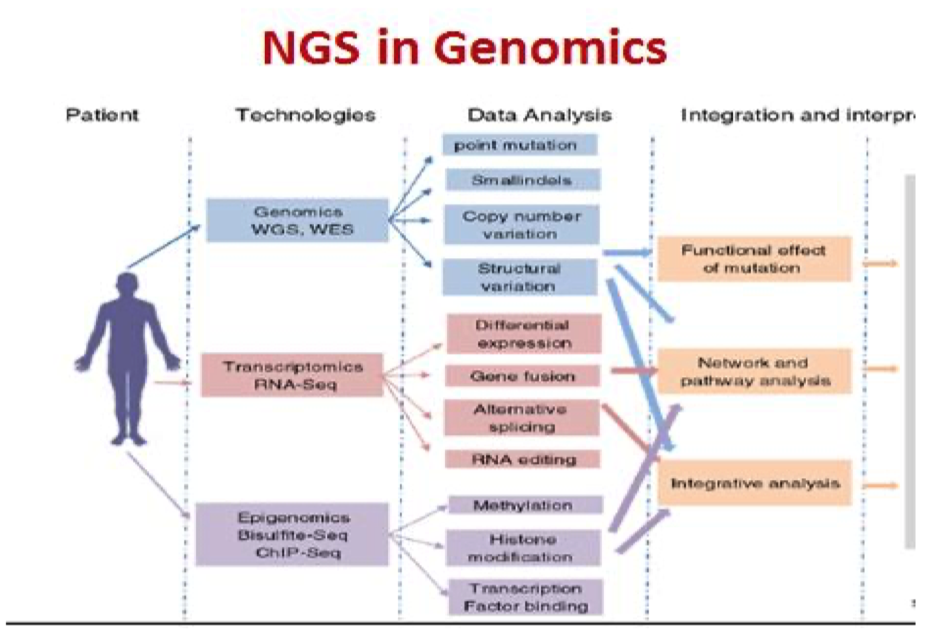
\includegraphics[width=\textwidth]{NGS_data}
  \caption[NGS data analysis classification]{
    NGS data analysis classification. The figure is from \url{http://www.biostat.jhsph.edu/~khansen/enar2012.html}.
  }
  \label{fig:NGS_data}
\end{figure}

Apart from multiple genomics data types generated from modern technologies, these data has their own underlying characteristics. Genomic annotation databases contains information about biological pathways and functional gene sets indicating a group of genes working collectively on one particular functionality. Examples of such annotation data bases are molecular signature database (MSigDB), gene ontology databases such as KEGG and reactome, and the chromosome on which a gene is located. There are also summary statistics like p-values, odds ratios, hazard ratios from external studies with related objective on the same set of genomics data. These information highlights the characteristics of genomic features, which are the features of genomic features. We call them meta-features from here and after. The meta-features reveal information on two fundamental characteristics of genomics, grouping and ordering. Gene annotations provide grouping information related to disease traits, while summary statistics provide ordering of genomic features, which indicates the importance of the features for a class of disease. 

Among the more important uses of these discoveries is providing detailed, mechanistic insight into the molecular pathogenesis of disease states. The two primary avenues of utilizing this explosion in genomics information for the purpose of improving clinical practices are in (1) prediction of disease prognostics, pharmacogenetic response, and disease severity/trajectory (2) prediction of treatment effects on individuals with certain genomic profiles and clinical features. Much of the variation in disease course, severity, and response to medication is reflective of the underlying genomic profile existing in each individual, offering the opportunity for genomics to facilitate early treatment, preventative medicine, preemptive selection of efficacious drugs, and more accurate estimation of risk for those thought to be at intermediate risk using traditional factors.

With the huge amount of genomics data in multiple categories, and ever growing annotation databases, the purpose of this thesis is to integrate multiple types of genomics data, meta-features into predictive modeling process, in the hope of improving model prediction performance, producing interpretable results (feature-selection).

\section{Genomics-based prediction of disease traits}
\label{sec:Prediction}
In the contest of discovering disease prognostic factors, predictive signals, predictive models are methods designed to use clinical, genomics, or other types of data for the purpose of forecasting a medical trait. Predictive models are most beneficial when they yield actionable and personalized results. They are of reduced value  if they only substantially modify medical decisions for a small fraction of the patient population. Therefore, the ideal genomics-based predictive model for clinical applications (1) substantially modifies the probability of medical traits upon which medical decisions based compared to that obtained from existing clinical assessment and tests, and (2) impacts a large fraction of individuals to whom it is applied and provides improved outcomes. Given that for many disease with multiple treatment strategies, accurate prediction of disease traits can play a critical role in determining robust clinical care that may avert severe disease, prolong survival, or even prevent disease onset. 

In this thesis, the focus is on cancer genomics applications. As the advent of genetic testing in tumor cells, through harnessing the throughput and read depth of NGS platforms, it has enabled detailed and clinically actionable molecular pathology genetic tests for numerous cancers. Multiplex sequencing-based assays for biopsies compared to normal tissue are now available and have demonstrated usefulness in augmenting many clinical decisions.

We give a brief overview of some of the high profile predictive modeling techniques for genomics. 

\subsection{Genome-wide association studies}
In an attempt to develop such predictive models, many have used genome-wide association study (GWAS). It is an approach used in genetics research to associate specific genetic variations with particular diseases \citep{manolio2010genomewide}. The method involves scanning the genomes from many different people and looking for genetic markers that can be used to predict the presence of a disease. Those genetic markers, either used alone or combined with traditional non-genetic risk prediction, have the potential to improve risk-prediction accuracy, which might benefit clinical diagnose and personalized treatment.

To carry out a genome-wide association study, two groups of subjects are identified: people with the disease being studied (cases) and similar people without the disease (controls); or people with different phenotypes for a particular trait, for example blood pressure, are identified. Each subject's complete set of DNA, genome is acquired and microarray chip technology or WGS, WES are applied to obtain common genetic variations, SNPs. It scans the entire genome to find statistically significant variations that are associated with the disease, using some form of family-wise error rate control.  

The discovery of genetic markers for the prediction of disease traits is entirely dependent on the underlying genetic model that gives rise to the trait. That is, the number of loci and the frequency and penetrance of predisposing alleles determine both the likelihood of identifying causal markers and the clinical utility of using those markers in a patient population. For example, monogenic disorders are very likely fully penetrant with allele frequencies that are not exceedingly rare, therefore, genetic tests for such diseases have clinical applications provided that disease prevention or disease trait dependent treatment exists. On the other hand, there are complex diseases that follow, e.g., weakly penetrant alleles, several hundreds to thousands loci, ubiquitous epigenetic effects, gene-environment interactions, or some combination hence, directly impacts the identification of predictive markers. GWAS interrogate the common allelic architecture for disease traits, whereas sequencing-based studies in families can facilitate the discovery of rare disease-associated variants, but are not optimal for identifying ancestral disease-predisposing alleles. Therefore, it is reasonable to expect that genetic markers from GWAS may apply to a large segment of individuals, but with a mild impact on the probability of disease traits.

\subsection{Regression}
Regression methods, linear models, are common techniques for constructing predictive models. For quantitative traits, it is linear regression; for dichotomous traits, logistic regression is deployed; for survival traits, Cox's proportional hazards regression, parametric regression models with various survival time distribution assumptions are for choices. Regression methods construct likelihood functions based on linear predictors. The input is a response vector $\bm{Y}$ of length $n$ (for survival outcomes, it is a response matrix of dimension $n \times 2$, survival time and censoring status) and a data/design matrix $\bm{X}$ of dimension $n \times p$, where $n$ is the number of independent samples, $p$ is the number of features. Then the linear predictors for each of the $n$ samples are defined as $\bm{\beta}^T\bm{x}_i$, where $\bm{x}_i$ is the features for the $i$th sample, $\bm{\beta}$ is the regression coefficients to be estimated. Negative log likelihood for each of the outcome types are listed below, i.e, the optimization problems for each of the regression models:
\begin{align}
    &\min_{\bm{\beta}} \left\{\frac{1}{2n} \sum_{i=1}^{n} (y_i-\bm{\beta}^T\bm{x}_i)^2 \right\}, \qquad\qquad\qquad\quad\;\: \text{linear regression} \label{eq1.1} \\
    &\min_{\bm{\beta}} \left\{-\frac{1}{n} \sum_{i=1}^{n} \left[y_i\bm{\beta}^T\bm{x}_i-\ln(1+e^{\bm{\beta}^T\bm{x}_i})\right]\right\}, \qquad \text{logistic regression} \label{eq1.2}
\end{align}
Cox's proportional hazards regression will be showed in detail in the following sections as the main medical traits to be dealt with. Incorporation of covariates and interaction effects are possible with regression, as opposed to GWAS, risk predictions are given by effect sizes of each significant hits.

There are several assumptions made when applying regression. First, the number of features $p$ should be less than the number of samples $n$ for the model to be able to fit. However, this is usually not the case in genomics study. DNA information are typically acquired by tissue biopsy in cancer patients. The biopsies could be highly invasive depending on the location of tumors, hence not feasible for everyone. Also, there are concerns for DNA sequencing cost. As a result, the number of samples is small to moderate at best, typical number ranges from hundreds to thousands. On the contrary, the number of genomic features is huge. There may be tens and hundreds of thousands genetic variations. If there are multiple types genomics including gene expressions, methylations and so on, the number is even larger. Therefore, genomics data are high dimensional ($p>>n$) in most cases. Multicollinearity between nearby markers is another serious concern. Highly correlated markers should have similar regression coefficients (negatively correlated markers have opposite sign, but similar in magnitude), i.e., a group of correlated markers share the group effect size equally. But in regression, the coefficient estimates are highly unstable given high correlation. Other concerns include marker-marker interactions, missing data. 

\subsection{Other machine learning methods}
Diagnosis and prognostic of disease traits with genomics information are classification and clustering problems within machine learning. Therefore, methods such as tree-based including random forest, gradient boosting machines, support vector machines, neural networks can be applied to these tasks. One of the applications in this category is Bayesian networks resulted from graph theory and applied probability \citep{jordan2004graphical}. Take a simplified version as an example, if the genomic features can be reasonably assumed independent conditional on disease traits, the network reduced to a naive Bayes model. Given a set of $p$ genomic features, the posterior probability of disease trait is:
\begin{align*}
    P(D|\cap_{i=1}^n G_i)&=\frac{P(\cap_{i=1}^n G_i|D)P(D)}{P(\cap_{i=1}^n G_i)} \\
    &=\frac{P(D=1)\prod_{i=1}^n P(G_i|D=1)}{P(D=1)\prod_{i=1}^n P(G_i|D=1)P(D=0)\prod_{i=1}^n P(G_i|D=0)}
\end{align*}
This carries some interpretability since the posterior probability tells some stories of how the genomic features contribute to disease traits. However, it is not as flexible in learning underlying non-linear patterns as its counterparts, tree-based, neural networks. It learns quadratic pattern and linear pattern when assuming equal variance of $G_i|D$, which shares some similarity with quadratic/linear discriminant analysis.

\subsection{Comparison of predictive methods in genomics}
Considering the high-dimensionality of genomics data, every genomic feature contribute a little to none effect to disease traits. Hence, there is not much effect either to contribute to square, square root of genomic features, etc., the non-linear patterns of features. Gradient boosting machine, neural network are superior when sample size is large, since there is enough information for them to explore complicated non-linear patterns. On the other hand, regression represents the genomic feature effects very well. Regression coefficients are effects to disease traits, they can be small to zero. This is the reason why regression is still the most widely used model in genomics, instead of tree-based methods and neural networks, despite their huge success in other areas.

GWAS scanned the whole genome one at a time to find significant hits after controlling for family-wise error rate, typically controlling for false discovery rate to allow more power to detect associated SNPs. With GWAS, only effect sizes of single signals are given, while regression has the ability to build a multivariate model for all detected signals and other covariates to be controlled, and also makes it possible to explore gene-gene, gene-environment interactions. However, in most cases, the combined effects of genetic markers found by GWAS explain a small proportion of inter individual differences in genetic risk. In part, this reflects lack of power of standard GWAS to detect small effect markers. A number of studies have shown that prediction accuracy can be increased by including in the model markers that may not show significant association at the marginal level, e.g., \citep{allen2010hundreds}. This brings out the key question in building predictive models in genomics, feature selection: which genomic features are most effective in determining the disease traits and should therefore be included in a predictive model.

The goal is to build a predictive model including genomic features collectively contribute most to disease trait, so as to maximize model's predictive power. One strategy is to include all genomics information at hand, and let the model decide which features are in the model to achieve optimal prediction performance. We know regression cannot be fit with high-dimensional data. Therefore, regularization need to be introduced. 

\section{Regularized regression}
Considering a linear regression, equation \eqref{eq1.1}, the solution to it is the ordinary least square (OLS), $\hat{\bm{\beta}}=(\bm{X}^T\bm{X})^{-1}\bm{X}^T\bm{Y}$. If $\bm{X}_{n\times p}$ is high-dimensional, $p>n$, the highest rank of matrix $(\bm{X}^T\bm{X})_{p\times p}$ is $\min(p,n)=n$, so it is a singular matrix. Mathematically, there is no solution to $\bm{\beta}$. Intuitively, the model is too complex to fit because there is not enough data. Regularization is a technique to control model complexity, by shrinking the regression coefficients. Regularized regression can be written as:
\begin{equation}
    \min_{\bm{\beta}} \left\{\ell(\bm{\beta)} + \lambda P(\bm{\beta)}\right\}, \label{eq1.3}
\end{equation}
where $\ell(\bm{\beta)}$ is the loss function/negative log likelihood. $P(\bm{\beta)}$ is the regularization/penalty function, which penalizes regression coefficients so that the estimates of coefficients shrink, making the model simpler.  $\lambda \geq0$ is a hyperparameter that controls amount of shrinkage, thus controls the model complexity. There are many type of penalty functions, we will look at some of the high profile types of regularization.

\subsection{Ridge regression}
Ridge regression is proposed by \cite{hoerl1970ridge}. It shrinks the regression coefficients by imposing a regularization/penalty on their size. The ridge coefficients minimize a regularized loss function,
\begin{equation}
    \min_{\bm{\beta}} \left\{ \ell(\bm{\beta})+\lambda\|\bm{\beta}\|_2^2  \right\}. \label{eq1.4}
\end{equation}
The larger the value of $\lambda$, the greater the amount of shrinkage on coefficients $\bm{\beta}$. The coefficients are shrunk toward zero. An equivalent way to write the ridge problem is 
\begin{equation}
    \begin{aligned}
    &\min_{\bm{\beta}} \ell(\bm{\beta}), \\
    &\text{subject to} \qquad \|\bm{\beta}\|_2^2 \leq t, \label{eq1.5}
    \end{aligned}
\end{equation}
which makes explicit the size constraint on the coefficients. There is a one-to-one correspondence between the parameters $\lambda$ and $t$. Where there are many correlated features in a standard regression model, their coefficients can be unstable due to high variance. By imposing a size constraint, the problem is alleviated. 

The solution to the ridge optimization problem is $\hat{\bm{\beta}}^{ridge}=(\bm{X}^T\bm{X}+\lambda \bm{I})^{-1}\bm{X}^T\bm{Y}$. Like the OLS solution, ridge regression solution is also a linear function of outcome $\bm{Y}$. It adds a positive constant $\lambda$ to the diagonal of $\bm{X}^T\bm{X}$ before inversion, making the matrix nonsingular even if $\bm{X}^T\bm{X}$ is not of full rank (high-dimensional setting). This is how ridge regression fit high-dimensional data and other ill-formed design matrix $\bm{X}$. In the case of orthonormal column spaces of $\bm{X}$, the ridge solution becomes a scaled version of the OLS solution, i.e., $\hat{\bm{\beta}}^{ridge}=\frac{1}{1+\lambda}\hat{\bm{\beta}}^{OLS}$, shrinking the coefficients by a fraction of $1+\lambda$. If the column spaces of $\bm{X}$ are not othonormal, ridge regression shrinks the directions with smallest variances the most. Those directions are in fact the principle components directions of $\bm{X}$. The first principle component has the largest sample variance (eigen value) amongst all normalized linear combinations of the columns of $\bm{X}$. Subsequent principal components have maximum variance subject to being orthogonal to the earlier ones. Hence, the small eigen value principle components directions are shrunk the most. 

Ridge regression has a Bayesian interpretation, assuming linear regression:
\begin{align*}
    &\bm{Y}|\bm{\beta};\bm{X} \sim N(\bm{X\beta}, \sigma^2\bm{I}), \\
    &\pi(\bm{\beta}) \sim N(0, \gamma^2\bm{I}).
\end{align*}
Both likelihood and prior are normal, therefore, the posterior distribution is also a normal. Because normal is its own conjugate family. The negative log posterior density of $\bm{\beta}$ is equal to the expression in equation \eqref{eq1.4}, with $\lambda=\sigma^2/\gamma^2$. Thus the ridge estimate is the mean and mode of the posterior distribution. In genomics, Bayesian ridge regression is the motivation of genomic best linear unbiased predictor (G-BLUP) \citep{de2013prediction}. 

Ridge regression shrinks coefficients toward zero, but never to exactly zero. In other words, it doesn't perform feature selection in terms of magnitude of regression coefficients. If coefficients shrink to zero, these features are no longer in the model, and thus not associated with outcome. Features with larger coefficients in magnitude, weather positive or negative, are strongly associated with outcome. However, ridge regularization is a widely used technique for controlling model complexity to balance the trade-off between bias and variance. The more complex the model, the less bias, but the larger variance, and vice versa. It is used in neural networks and gradient boosting machines, where it is known as weight decay.    

\subsection{Sparse regularized regression and feature selection}
\subsubsection{The Lasso}
Proposed by \citep{tibshirani1996regression}, the lasso is a regularization method like ridge, but performs feature selection. The lasso optimization problem, Lagrangian form, is defined as 
\begin{equation}
    \min_{\bm{\beta}} \left\{ \ell(\bm{\beta})+\lambda\|\bm{\beta}\|_1  \right\}. \label{eq1.6}
\end{equation}
It can also be written in the equivalent constrained optimization problem just like ridge,
\begin{equation}
    \begin{aligned}
    &\min_{\bm{\beta}} \ell(\bm{\beta}), \\
    &\text{subject to} \qquad \|\bm{\beta}\|_1 \leq t. \label{eq1.7}
    \end{aligned}
\end{equation}
The similarity to the ridge regression is the $L_2$ norm penalty function for ridge is replaced by $L_1$ norm penalty function for the lasso. The term sparse refers to a model with few nonzero coefficients. A key property of the lasso is its ability to yield sparse solutions. Lets look at the lasso estimator for linear regression. For the $j^{th}$ feature, i.e, the $j^{th}$ element of coefficients vector $\bm{\beta}$, the coordinate-wise update, for standardized features with mean 0 and variance 1, has the form
\begin{equation}
    \hat{\beta}_j^{lasso}=S(\frac{1}{n}\sum_{i=1}^{n}x_{ij}r_i^{(j)}, \lambda) \label{eq1.8}
\end{equation}
where 
\begin{itemize}
    \item $r_i^{(j)} = y_i-\sum_{l\neq j}x_{il}\hat{\beta}_l$ is the partial residual which removes from the outcome the current fit from all but the $j^{th}$ predictor. Because features are usually standardized to make the shrinkage comparable, $\frac{1}{n}\sum_{i=1}^{n}x_{ij}r_i^{(j)}$ is the simple least squares solution when fitting this partial residual to $x_{ij}$.
    \item $S(x, \lambda)$ is the soft-thresholding operator defined as 
    \begin{equation}
        \text{sign}(x)(|x|-\lambda)_+ = 
            \begin{cases}
                x-\lambda & \text{if $x>0$ and $\lambda<|x|$}\\
                x+\lambda & \text{if $x<0$ and $\lambda<|x|$}\\
                0 & \text{if $\lambda \geq |x|$}
            \end{cases} \label{eq1.9}      
    \end{equation}
\end{itemize}
One can derive the results using the notion of subgradients, the detailed derivation of coordinate descent are described in \cite{friedman2007pathwise}. Notice the lasso solution shrinks the regression coefficient (solution of least squares, $\frac{1}{n}\sum_{i=1}^{n}x_{ij}r_i^{(j)}$) by an amount of $\lambda$, as long as its magnitude/absolute value is larger than $\lambda$. For the features having smaller effect sizes than $\lambda$, they are shrunk to 0, thus being excluded to the model (Figure \ref{fig:soft_threshold}). This is the main difference between ridge and the lasso, while ridge regression does a proportional shrinkage, lasso translates each coefficient by a constant $\lambda$, truncating at zero. Therefore, the lasso has the ability to perform feature selection by excluding unimportant features. In this way, the lasso model is more parsimonious, more interpretable, compared to ridge, which keeps all the features in the model.
\begin{figure}[tbh]
  \centering
  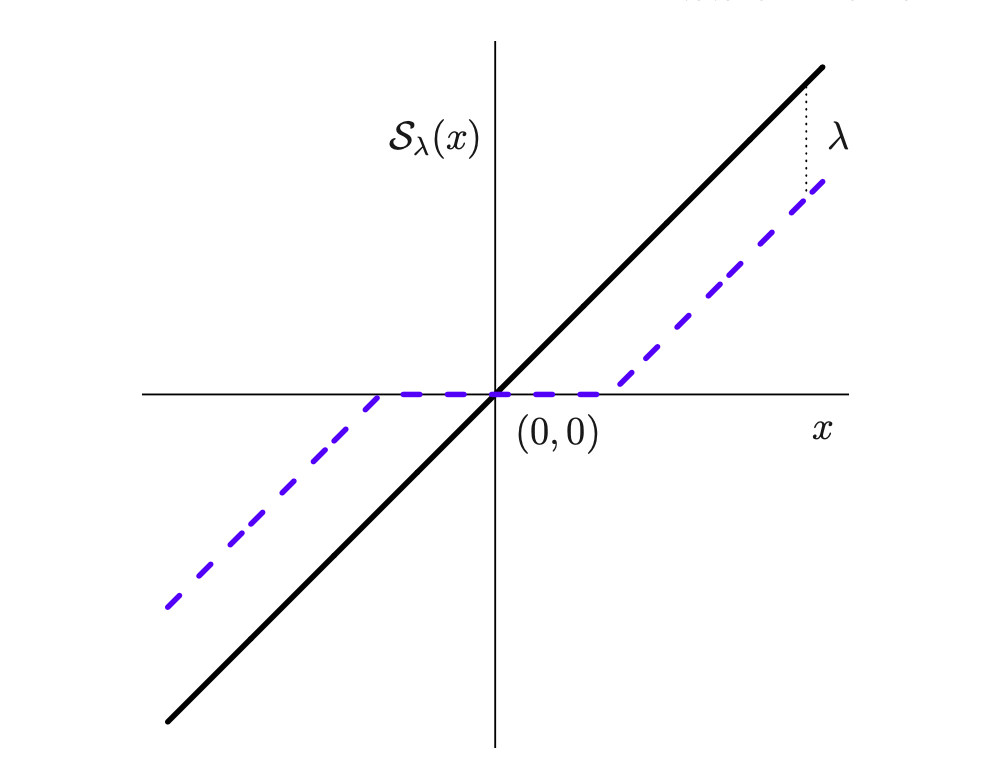
\includegraphics[scale=0.6]{soft_threshold}
  \caption[Soft thresholding function $S(x, \lambda)=\text{sign}(x)(|x|-\lambda)_+$]{
    Soft thresholding function $S(x, \lambda)=\text{sign}(x)(|x|-\lambda)_+$. The figure is from \cite{hastie2019statistical}. The blue broken line is the soft threshoding estimator, along with the $45^{\circ}$ line in black.
  }
  \label{fig:soft_threshold}
\end{figure}

There are some important properties of the lasso in addition to feature selection.
\begin{itemize}
    \item Just like ridge regression, the lasso also has an Bayesian interpretation. The prior distribution of $\bm{\beta}$ is double exponential/Laplace for the lasso, instead of normal for ridge.
    \item Degrees of freedom: Suppose there are $p$ features, fitting a linear regression using only a subset of $k$ of these features, if these $k$ features were chosen without regard to the outcome, the procedure spends $k$ degrees of freedom. However, if the $k$ features were chose using knowledge of the outcome, for example best subset selection, then the fitting procedure spends more than $k$ degrees of freedom. Such a fitting strategy is adaptive, as well as the lasso. The lasso, with a fixed penalty parameter $\lambda$, the number of nonzero coefficients $k_\lambda$ is an unbiased estimate of the degrees of freedom \citep{zou2007degrees, tibshirani2012degrees}. The reason that lasso has exactly $k$ degrees of freedom rather than larger than $k$ is that it not only selects features which inflates the degrees of freedom, but also shrinks the coefficients. This result gives us a qualitative measure of the amount of fitting having been done at any point along the lasso path.
    \item The number of nonzero coefficients is at most $n$, the sample size, when the data is high dimensional, $p>n$.
    \item Assume that the underlying true signal is sparse, the lasso recovers the true signals well. If the underlying truth is not sparse, the lasso does not work well. 
\end{itemize}

\subsubsection{The elastic net}
Proposed by \cite{zou2005regularization}, the elastic net makes a compromise between the ridge and the lasso; it solves the convex optimization problem
\begin{equation}
    \min_{\beta} \left\{ \ell(\bm{\beta})+\lambda\left[\frac{1}{2}(1-c)\|\bm{\beta}\|_2^2+c\|\bm{\beta}\|_1\right] \label{eq1.10} \right\} 
\end{equation}
where $c\in [0,1]$ is a parameter that controls whether the penalty function to be more close to lasso or more close to ridge. When $c=1$, it reduces to $L_1$ norm, lasso penalty; when $c=0$, it reduces to squared $L_2$ norm, ridge penalty. The coordinate-wise update for the elastic net linear regression, again assuming the features are standardized to mean 0 and variance 1, is 
\begin{equation}
    \hat{\beta}_j^{enet} = \frac{S(\frac{1}{n}\sum_{i=1}^{n}x_{ij}r_i^{(j)}, \lambda c)}{1+\lambda(1-c)} \label{eq1.11}
\end{equation}
We can see the elastic net estimator shrinks the regression coefficients in the way of both lasso and ridge: it has the soft-thresholding portion truncating at $\lambda c$; it also shrink the coefficients proportionally with a factor of $1+\lambda(1-c)$. Hence, the elastic net shrinks the coefficients and some of them to exactly 0, so feature selection.

\subsection{Discussion of ridge regression, the lasso, the elastic net, and best subset selection}
Best subset selection finds for each $k\in\{0,1,2,\dots,p\}$ the subset of size $k$ that gives smallest residual sum of squares (validation error). Best subset selection linear regression is equivalent to $L_0$ constrained regression, when design matrix $\bm{X}$ is orthogonal:
\begin{equation}
\begin{aligned}
    &\min_{\bm{\beta}} \frac{1}{2n}\|\bm{Y}-\bm{X\beta}\|_2^2, \\
    &\text{subject to} \quad \|\bm{\beta}\|_0 \leq k, \label{eq1.12}
\end{aligned}
\end{equation}
where $\|\bm{\beta}\|_0=\sum_{j=1}^p I(\beta_j \neq 0)$, is defined as the number of nonzero coefficients. Strictly speaking, $L_0$ is not a norm because it does not have properties of a norm, but the naming and notation are widely used. The $L_0$ constraint penalizes the number of nonzero coefficients, instead of the magnitude of coefficients. This exactly describes the best subset selection setting. And because it does not shrink the coefficients, the $L_0$ estimates are unbiased, while other regularization estimates are biased toward 0. Although, best subset selection, or $L_0$ constrained regression is superior in coefficient estimation, feature selection, it does not have an efficient algorithm, when $\bm{X}$ is not orthogonal. If we want to select a best subset without knowing how many features should be included to be the best subset, $k$, then there are $2^p$ combinations of features need to be examined. In other words, there are no polynomial time algorithm to solve it; the problem is NP-hard. Many approximation methods have been proposed to solve the problem. Among them, iterative hard thresholding is well performed. The closed form hard thresholding solution for $L_0$ constrained linear regression when $\bm{X}$ is orthogonal is   
\begin{equation}
    \hat{\bm{\beta}}^{L_0}=H_{\sqrt{2\lambda}}(\frac{1}{n}\bm{X}^T\bm{Y}), \label{eq1.13}
\end{equation}
where $H_{\sqrt{2\lambda}}(\cdot)$ is the hard thresholding operator,
\begin{equation}
    H_{\sqrt{2\lambda}}(\frac{1}{n}\bm{X}^T\bm{Y})=
    \begin{cases}
        \frac{1}{n}\bm{X}^T\bm{Y} & \text{if $|\frac{1}{n}\bm{X}^T\bm{Y}|>\sqrt{2\lambda}$}, \\
        0 & \text{if $|\frac{1}{n}\bm{X}^T\bm{Y}|\leq\sqrt{2\lambda}$}.
    \end{cases}
\end{equation}
It does not shrink regression coefficients at all, but truncates at $\sqrt{2\lambda}$. This is in close relation to the soft thresholding estimator of lasso, equation \eqref{eq1.9}, which shrinks coefficients by the amount of $\lambda$ and truncates at $\lambda$. This is why hard thresholding is an unbiased estimator of regression coefficient. In fact, the lasso is one of many approximations to $L_0$ constrained problem. And it is the closest convex approximation to it, while $L_0$ is a nonconvex optimization problem. Figure \ref{fig:estimators} shows the estimators for best subset/$L_0$, ridge, and lasso in the case of orthonormal orthogonal $\bm{X}$. We can see the unbiased estimator of best subset; feature selection ability of best subset and lasso; and different shrinkage scheme between ridge and lasso.
\begin{figure}[tbh]
  \centering
  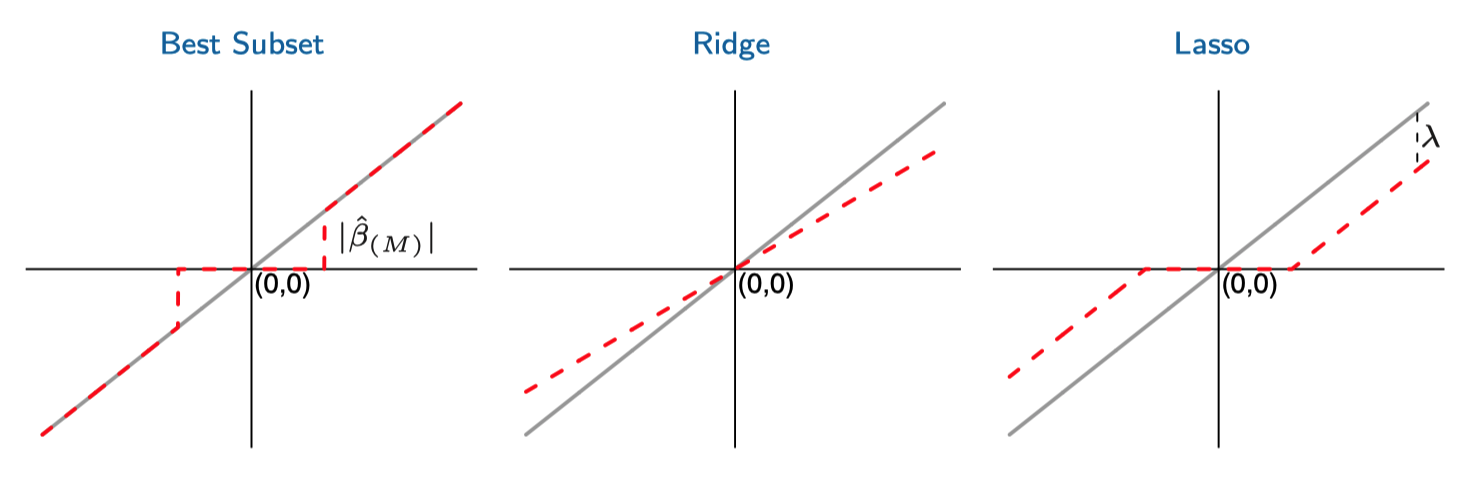
\includegraphics[scale=0.6]{estimator}
  \caption[Estimators of $\beta_j$ in the case of orthonormal columns of $\bm{X}$]{
    Estimators of $\beta_j$ for best subset, ridge, lasso, in the case of orthonormal columns of $\bm{X}$. Estimators are shown by broken red lines. The figure is from \cite{hastie2009elements}.
  }
  \label{fig:estimators}
\end{figure}

Ridge regression and the elastic net are also convex optimization problems. Since ridge, lasso and elastic net share this nice property, they have a highly efficient computational algorithm in pathwise coordinate descent \citep{friedman2007pathwise}. The algorithm solves the problems along a decreasing sequence of $\lambda$ values, for the purpose of tuning $\lambda$ via cross validation. Apart from giving a path of solutions, the algorithm exploits warm start, which initializes $\hat{\bm{\beta}}$ with the solutions of previous $\lambda$ value. This works because convex objective functions have continuous solutions along the path. By starting at previous solutions, coordinate descent updates need less iterations, thus leads to a more efficient and stable algorithm. On the other hand, iterative hard thresholding is not as efficient, and only guarantees to reach local minimums due to $L_0$'s nonconvexity. 

The lasso does not deal with highly correlated features very well; the solutions tend to be unstable. If there is a group of variables among which the pairwise correlations are very high, then the lasso tends to select only one variable from the group and does not care which one is selected. Ridge regression is known to shrink the coefficients of correlated features towards each other, allowing them to borrow strength from each other. In the extreme case of $k$ identical features, they each get identical coefficients with $1/k$ the size that any single one would get if fit alone. The elastic net is a combination of ridge and lasso. It selects features like the lasso, and shrinks together the coefficients of correlated features like ridge. As $c$ increases from 0 to 1, for a given $\lambda$, the sparsity of the elastic net solution, i.e., the number of coefficients equal to zero, increases monotonically from 0 to the sparsity of the lasso solution. 

\subsection{Nonconvex regularized regression}
Ridge regression, the lasso, the elastic net are all convex optimization problems. There are stable and efficient algorithms to solve it. And they always reach their global minimum solutions. Because of these, they are widely used for regularization, controlling model complexity. However, by moving from $L_2$ ridge to $L_1$ lasso, we have seen the lasso selects a subset of features to have nonzero coefficients, and shrinks them. When the number of features is large and the number of relevant features is small, this may not be enough. In order to reduce the set of chosen features sufficiently, lasso may end up over-shrinking the retained features. Nonconvex regularization leads to more sparse, less biased solutions. To see this, consider $L_q$ regularization,
\begin{equation}
    \min_{\bm{\beta}} \left\{ \frac{1}{2n}\|\bm{Y} - \bm{X\beta}\|_2^2 + \lambda \sum_{j=1}^{p}|\beta_j|^q \right\} \label{eq1.15}
\end{equation}
for $q\geq0$. It is the lasso for $q=1$, ridge for $q=2$. Figure \ref{fig:lq} displays $L_q$ regularization in the case of two inputs. For $0 \leq q <1$, the regularization is nonconvex, with the limiting $q=0$ corresponding to best subset selection. For these nonconvex constraints, they concentrate more mass in the coordinate directions, thus the solutions tend to be more sparse, and less shrinkage (biased toward 0). Unfortunately, along with nonconvexity comes combinatorial computational complexity and unstable algorithms. Alternatives nonconvex regularization have been proposed.
\begin{figure}[tbh]
  \centering
  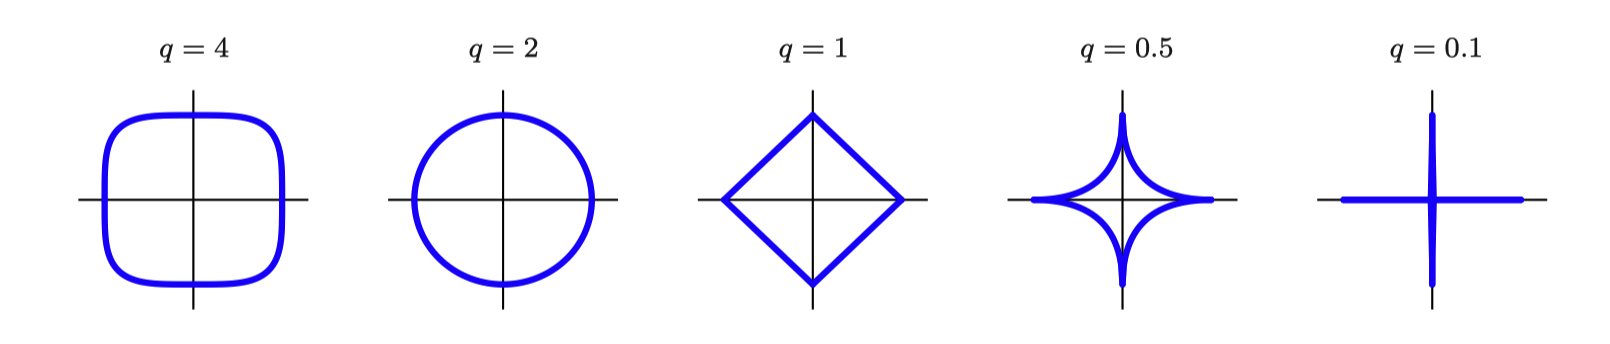
\includegraphics[width=\textwidth]{lq}
  \caption[Constraint regions $\sum_{j=1}^p|\beta_j|^q\leq1$ for different values of $q$] {
    Constraint regions $\sum_{j=1}^p|\beta_j|^q\leq1$ for different values of $q$. For $q<1$, the constraint region is nonconvex. The figure is from \cite{hastie2009elements}. 
  }
  \label{fig:lq}
\end{figure}

\subsubsection{Smoothed clipped absolute deviation penalty (SCAD) and minimax concave penalty (MCP)}
Proposed by \cite{fan2001variable}, the SCAD penalty defined on $[0, \infty)$ is given by (symmetric on $(-\infty, 0)$)
\begin{equation}
    P_{\lambda,\gamma}(\beta) = 
        \begin{cases}
            \lambda\beta & \text{if $\beta \leq \lambda$}\\
            \frac{\gamma\lambda\beta-0.5(\beta_2+\lambda^2)}{\gamma-1} & \text{if $\lambda<\beta\leq\gamma\lambda$}\\
            \frac{\lambda^2(\gamma^2-1)}{2(\gamma-1)} & \text{if $\beta>\gamma\lambda$}
        \end{cases} \label{eq1.16}      
\end{equation}
for $\lambda\geq0$ and $\gamma>2$. The univariate solution for a SCAD regularized simple linear regression coefficient is as follow
\begin{equation}
    \hat{\beta}=f_{SCAD}(z,\lambda,\gamma)= 
        \begin{cases}
            S(z,\lambda) & \text{if $|z|\leq 2\lambda$}\\
            \frac{S(z, \gamma\lambda/(\gamma-1))}{1-1/(\gamma-1)} & \text{if $2\lambda<|z|\leq\gamma\lambda$}\\
            z & \text{if $|z|>\gamma\lambda$}
        \end{cases} \label{eq1.17}      
\end{equation}
where $z=\frac{1}{n}\bm{X}^T\bm{Y}$ is the OLS solution.

Proposed by \cite{zhang2010nearly}, the MC+ penalty defined on $[0, \infty)$ is given by (symmetric on $(-\infty, 0)$)
\begin{equation}
    P_{\lambda,\gamma}(\beta) = 
        \begin{cases}
            \lambda\beta - \frac{\beta^2}{2\gamma} & \text{if $\beta \leq \gamma\lambda$}\\
            \frac{1}{2}\gamma\lambda^2 & \text{if $\beta>\gamma\lambda$}
        \end{cases} \label{eq1.18}      
\end{equation}
for $\lambda\geq0$ and $\gamma>1$. The univariate solution for a MC+ regularized simple linear regression coefficient is as follow
\begin{equation}
    \hat{\beta}=f_{MCP}(z,\lambda,\gamma)= 
        \begin{cases}
            \frac{S(z,\lambda)}{1-1/\gamma} & \text{if $|z|\leq \gamma\lambda$}\\
            z & \text{if $|z|>\gamma\lambda$}.
        \end{cases} \label{eq1.19}      
\end{equation}

The rational of SCAD and MCP is similar in that both penalties begin by applying same penalty as the lasso, and reduce the amount of penalty as the regression coefficient gets further away from zero. As a result of the penalty trend, when the coefficient is small in magnitude, it is shrunk to zero just like lasso; however, when the coefficient is large (larger than OLS solution), there is a transition region that shrinks the coefficient less than the lasso, and after the transition region, it is equal to the OLS solution without any shrinkage. This is a trend from less biased toward 0 to unbiased estimator, for those features with large effect sizes, thereby more likely to be associated with outcomes. Without the transition region, it is the hard thresholding estimator. The difference between SCAD and MCP is in the way they make transition. Figure \ref{fig:nonconvex_est} shows the trend of penalty functions of SCAD, MCP and their threshold functions. Indexed by nonconvexity parameter $\gamma$, it bridges the gap between lasso ($\gamma=\infty$) and best subset/hard threshold ($\gamma=2_+$ for SCAD $1_+$ for MCP).   
\begin{figure}[tbh]
  \centering
  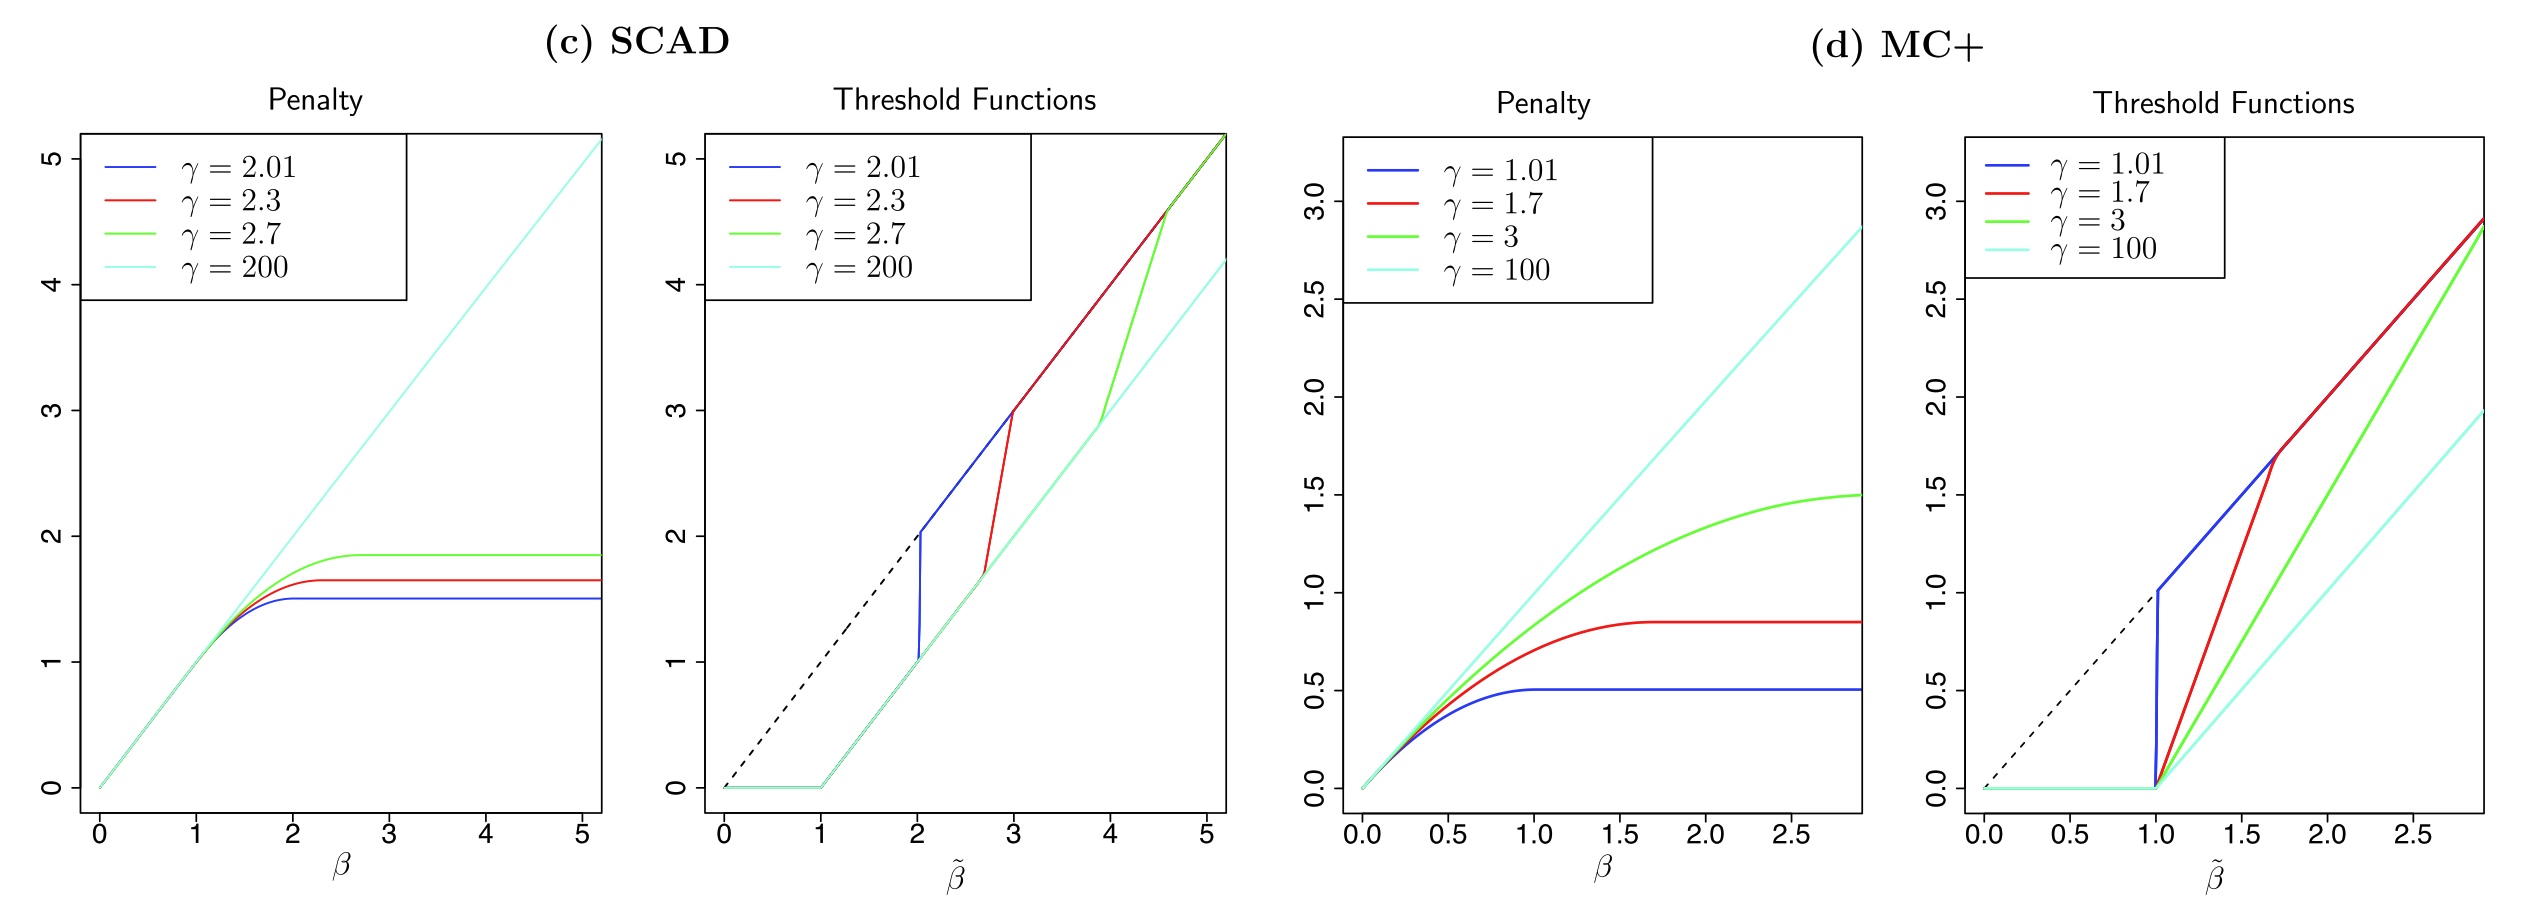
\includegraphics[width=\textwidth]{nonconvex_est}
  \caption[SCAD and MCP penalty functions and their corresponding threshold functions] {
    SCAD and MCP penalty functions and their corresponding threshold functions. Both are shown with $\lambda=1$ and different values for $\gamma$. The figure is from \cite{mazumder2011sparsenet}. 
  }
  \label{fig:nonconvex_est}
\end{figure}

The two nonconvex regularization techniques achieve less biased estimator, more sparse subset than the lasso. The choice of convex and nonconvex regularization depends on the application. For example, for a gene expression profile data, the underlying model is sparse but with a relatively large subset of features, the lasso is a better choice. Because with a large number of features in the model, say $1000-2000$, the direction of the feature coefficients are more meaningful rather than the magnitude of the coefficients. For a genetic association data, by which the underlying model only consists of a few markers, the accuracy of selection and unbiasedness of estimators are important. Hence, nonconvex regularization is a better suit in the situation.

We close the section by mentioning an approximation to $L_q$ ($0\leq q <1$) regularization that enjoys convex property.

\subsubsection{The adaptive lasso: approximation to nonconvex regularization}
Proposed by \cite{zou2006adaptive}, the adaptive lasso is a way of fitting models sparser than lasso. Using a pilot estimate $\tilde{\beta}$, the adaptive lasso has the form
\begin{equation}
    \min_{\bm{\beta}} \left\{ \frac{1}{2n}\|\bm{Y}-\bm{X\beta}\|_2^2+\lambda\sum_{j=1}^pw_j|\beta_j| \right\}, \label{eq1.20}
\end{equation}
where $w_j=1/|\tilde{\beta}_j|^v$. The adaptive lasso can be seen as an approximation to the $L_q$ regularization with $q=1-v$. We can see the adaptive lasso is convex in $\bm{\beta}$. Moreover, when the pilot estimates meet some regulatory conditions, the method recovers the true model under more general conditions than does the lasso. One can use least squares solution as the pilot estimate when $p<n$, univariate least squares solution when $p\geq n$. The indication is that, when least squares solution is small, the amount of penalty $w_j$ for feature $j$ is large, thereby $\hat{\beta}_j$ is more likely to be set to 0; when least squares solution is large, feature $j$ is penalized less (small $w_j$), then $\hat{\beta}_j$ is shrunk less, making it less likely to be 0 and less biased.